%
% einleitung.tex -- Beispiel-File für die Einleitung
%
% (c) 2020 Prof Dr Andreas Müller, Hochschule Rapperswil
%
\section{Gradient Descent\label{cg:section:steepest_descent}}
\rhead{Gradient Descent}

Um den CG-Algorithmus zu verstehen, ist es hilfreich zuerst die Steepest Descent Methode zu analysieren.
Steepest Descent ist eine bekannte Methode um iterativ ein Minimierungsproblem zu lösen.
Dabei wird immer eine gewisse Schrittweite weit entlang des Gradienten des Minimierungsproblems abgestiegen.
Eine Darstellung von einem 2-Dimensionalen Minimierungsproblem mit Gradient Descent findet sich in Abbildung \ref{cg:abb:steepest_descent}.

\begin{figure}
	\label{cg:abb:steepest_descent}
	\centering
	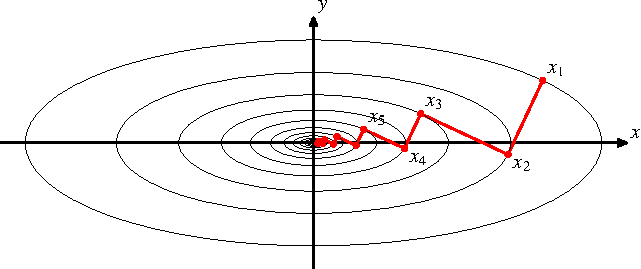
\includegraphics{papers/cg/images/descent-1}
	\caption{Gradient Descent für ellipsenförmige Niveaulinien (schlechte Konditionierung) in 2D. 
		Offensichtlich ist die Konvergenz schlecht. Abbildung aus dem Seminar Buch von 2014 \cite{cg:book:hpc}}.
\end{figure}

\subsection{Minimierungsproblem \label{cg:subsection:Minimierungsproblem}}

Eine Lösung für $x$ kann durch Minimieren von
\begin{equation}
\Phi(x) = \frac{1}{2} x^T A x - x^T b
\end{equation}
gefunden werden.
Der folgende Beweis zeigt, wieso dies ein sinnvoller Ansatz ist.

\begin{proof}[Beweis]
	Wir definieren eine zweite Variable $z = x + \lambda y$, was uns erlaubt die folgende Differenz auszurechnen
	\begin{align}
	\Phi(z) - \Phi(x) 
	&= 
	\frac{1}{2} \left(x + \lambda y\right) ^T A \left(x + \lambda y\right)  - \left(x + \lambda y\right) ^T b
	- 
	\frac{1}{2} x^T A x + x^T b 
	\\
	&= 
	\frac{1}{2} \left(x^T A x + x^T A \lambda y + \lambda y^T A x + \lambda y^T A \lambda y\right) 
	-
	x^T b - \lambda y^T b
	- 
	\frac{1}{2} x^T A x + x^T b .	
	\end{align}
	Da $A$ symmetrisch ist, können die Terme $x^T A \lambda y$ und $\lambda y^T A x$ zusammengefasst werden (analog zur binomischen Formel)
	\begin{align}
	\Phi(z) - \Phi(x) 
	&= 
	\frac{1}{2}\cancel{ x^T A x} + x^T A \lambda y + \frac{1}{2} \lambda y^T A \lambda y
	-
	\bcancel{x^T b} - \lambda y^T b
	- 
	\frac{1}{2}\cancel{ x^T A x} + \bcancel{x^T b} \\
	&=
	\lambda x^T A y	+ \frac{1}{2} {\lambda}^2 y^T A y - \lambda y^T b \\
	&=
	\frac{{\lambda}^2}{2} y^T A y + \lambda y^T \left(Ax -b \right) .
	\end{align}
	Nun können wir den Beweis führen, indem wir $\Phi(z) \ge \Phi(x)$ setzen (da $\Phi(x)$ ja minimiert wird)
	\begin{align}
	\Phi(z) &\ge \Phi(x) 
	\\
	\Phi(z) &= \frac{{\lambda}^2}{2} y^T A y + \lambda y^T \left(Ax -b \right) + \Phi(x) 
	\\
	0 &\le \frac{{\lambda}^2}{2} y^T A y + \lambda y^T \left(Ax - b \right) \quad \forall \quad y \in \mathbb{R}^N  .
	\end{align}
	Der erste Term ist dabei quadratisch in $\lambda$, $A$ ist positiv definit und somit ist immer $\frac{{\lambda}^2}{2} y^T A y \ge 0$.
	Beim zweiten Term ist diese Bedingung nur erfüllt für alle $y$, wenn $Ax - b = 0$.
	Damit ist bewiesen, dass eine Lösung für die Gleichung $Ax = b$ durch Minimierung von $\Phi(x)$ gefunden wird.
\end{proof}

\subsection{Anwendung von Gradient Descent}
